\documentclass[11pt, a4paper, chapterprefix=false]{scrreprt}
\RedeclareSectionCommand[beforeskip=-1\baselineskip]{chapter}
\usepackage[a4paper, left=3cm, right=3cm, top=2cm]{geometry}
\usepackage{palatino, url}
\usepackage[ngermanb]{babel}
\usepackage[utf8]{inputenc}
%\setlength{\parindent}{0cm}
\usepackage{graphicx}
\usepackage{setspace}
\onehalfspacing
\usepackage{amsfonts}
\bibliographystyle{plain}

\begin{document}
	
	%Teteldeklaration und Erstellung
	\begin{titlepage}
	\author{Dipl. -Met K L \\ 5xxxxxx} 
	\title{\textit{Seminar 01909}\\ Maßnahmen zur Absicherung von privaten und kleinen und Unternehmensnetzwerken: \\ Virtuelle private Netzwerke und virtuelle LANs } 
	\date{Wintersemester 2018/19} 
	\maketitle
	\end{titlepage}
	%\newpage 
	%\thispagestyle{empty}
	%\quad 
	\newpage
	
	%Inhaltsverzeichnis
	
	\tableofcontents
	
	%Kapitel
	\setcounter{page}{1}
	
	\chapter{Einleitung}



Die Kommunikation über das Internet, die Verfügbarkeit von digitalen Medien nahezu jederzeit und überall und das Anhäufen von digitalen Daten  sind  heute Teil des Alltags, sowohl im privten wie auch im geschäftlichen Bereich. Auch für Unternehmen  sind das Netzwerk und das Internet ein wichtiger wirtschaftlicher Faktor geworden \cite{lipp2007vpn}. Dabei sind  Flexibilität und Sicherheit von großer Bedeutung, allerdings spielen gerade in einem Unternehmen auch die Kosten eine wichtige Rolle. Durch virtuelle Netzwerkstrukturen wie virtuelles LAN (VLAN) und virtuelle Private Netze (VPN) ist es möglich, kostengünstige Lösungen zu schaffen. 

Dem Aspekt der Sicherheit muss dabei besondere Beachtung geschenkt werden, da Angriffe auf Firmennetze erheblichen finanziellen Schaden verursachen können.\\  

Eine Studie des WIK (Wissenschaftliches Institut für Infrastruktur und Kommunikationsdienste) \cite{wik2017KMU} ergab, dass zwar 64 \% der kleinen Unternehmen\footnote{Unternehmen mit bis zu 49 Mitarbeitern werden hier als kleine Unternehmen bezeichnet.} in Deutschland angeben, IT-Sicherheit habe eine hohe Bedeutung, eine Sicherheitsanalyse aber nur von $20\; \%$ durchgeführt wurde.
Dabei benutzen 94 \% der kleinen Unternehmen laut dieser Umfrage PC-Arbeitsplätze mit Internetzugang und in  75 \%  kommen mobile Endgeräte wie Smartphones, Notebooks und Tablets zum Einsatz. Gleichzeitig geben nur 31 \% der kleinen Unternehmen an, VPN zu nutzen. Bereits Virenangriffen ausgesetzt waren 53 \% der Unternehmen. 





  %Im Jahr 2016 gaben $50\%$ der kleinen Unternehmen an schon mal einen Cyberangriff festgestellt zu haben. Der Prozetnsatz wächst mit der Unternehmensgröße weiter an\footnote{Cybersicherheits-Umfrage der Allianz für Cybersicherheit 2016}. 




Im Folgenden sollen die virtuellen Netzwerkstrukturen VPN und VLAN vorgestellt werden. In Kapitel 2 soll zunächst kurz ein Überblick über des Aufbau eines sicheren Unternehmensnetzwerks gegeben werden. Kapitel 3 gibt eine Einführung in das Thema VLAN und der damit verbundenen logischen Segmentierung des lokalen Netzes eines Unternehmens. Im vierten Kapitel wird daraufhin die virtuelle Standorterweiterung eines lokalen Unternehmensnetzes, bzw. der Zugriff aus der Ferne durch VPN vorgestellt. 
Schließlich bietet Kapitel 5 eine kurze Zusammenfassung und einen Ausblick. 































%Die Digitalisierung bringt sowohl für Privathaushalte, als auch für Unternehmen viele neue Möglichkeiten. Durch die zunehmende Vernetzung ergeben sich aber auch vielfältige Angriffsmöglichkeiten, die die Sicherheit von Privathaushalten und Unternehmen bedrohen. IT-Sicherheit wird auch in kleinen Unternehmen zunehmend wichtiger, die Umsetzung dieser fällt jedoch gerade kleinen Unternehmen häufig noch schwer. Eine Studie des WIK (Wissenschaftliches Institut für Infrastruktur und Kommunikationsdienste} ergab, dass zwar $64\%$ der kleinen Unternehmen in Deutschland angeben IT-Sicherheit habe eine hohe Bedeutung, eine Sicherheitsanalyse aber nur von $20\%$ durchgeführt wurde \cite{wik2017KMU}.   


%....%
%Das Netzwerk und die Internetanbindung wurden in den letzten Jahren zu einem wichtigen Faktor, auch für den wirtschaftlichen Erfolg eines Unternehmens \cite{lipp2007vpn}.


	
	\chapter{Basisarchitektur für ein sicheres Netzwerk}
Die Grundarchitektur für ein sicheres Netzwerk umfasst laut Bundesamt für Sicherheit in der Informationstechnik (BSI) 3 Zonen \cite{isi-lana}: 
\begin{itemize}
	\item das Interne Netz 
	\item das Sicherheitsgateway
	\item sowie die Internet Anbindung	
\end{itemize}
Abbildung \ref{grundarch} zeigt diesen Aufbau. Das \emph{Local Area Network} (\emph{LAN}) besteht aus mehreren, physikalisch durch einen Paketfilter getrennten, Subnetzen. Hier sollten sich zumindest die Server und die Clientrechner in eigenen Subnetzen befinden, sowie Rechner mit unterschiedlich hohem Schutzbedarf. 

\begin{figure}
	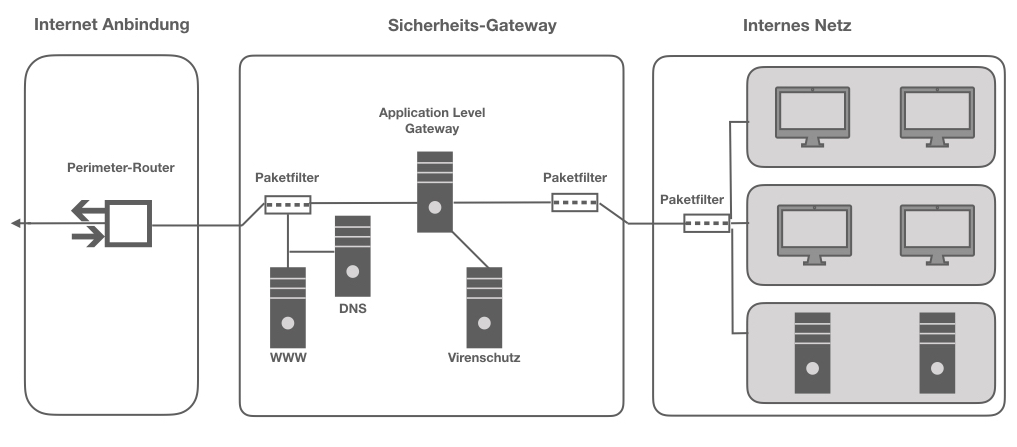
\includegraphics[width=\linewidth]{grundarchitektur}
	\caption{Grundarchitektur eines sicheren Netzwerkes}
	\label{grundarch}
\end{figure}

Die zwiete Zone, das Sicherheitsgateway, trennt die InternetAnbindung vom internen Firmennetz. Hier wird eine P-A-P Struktur empfohlen, bestehend aus einem Paketfilter auf der Seite des lokalen Netzes, sowie einem Paketfilter auf Seite des Internets, die jeweils die Kommunikation auf der dritten Schicht des Protokollstapel, der Vermittlungsschicht oder auch IP-Schicht, filtern. Der Paketfilter auf Seiten des LANs untersucht die nach außen gerichteten Pakete, der Paketfilter auf Seiten der Internetanbindung filtert die ankommenden IP-Pakete.

\begin{figure}
	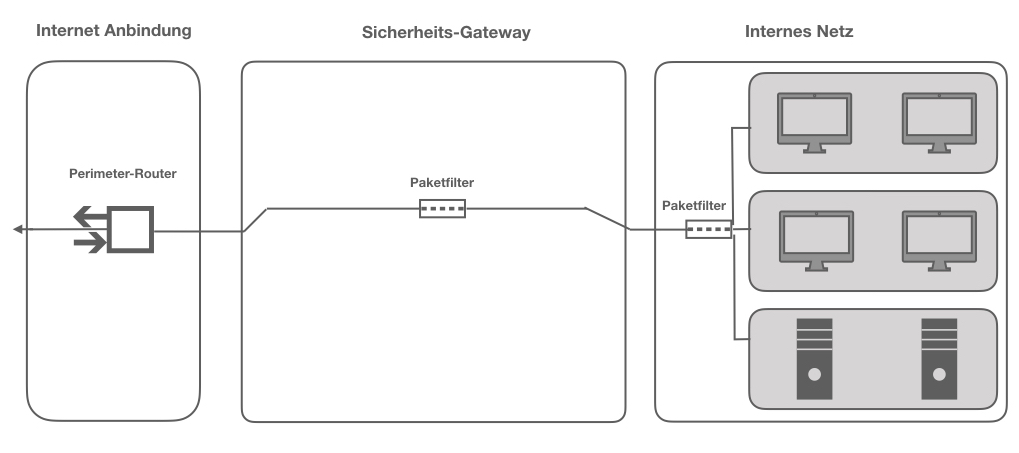
\includegraphics[width=\linewidth]{klUnternHoch.jpeg}
	\caption{Grundarchitektur für ein kleines Unternehmen mit normalem Schutzbedarf}
	\label{klUnorm}
\end{figure}

\begin{figure}
	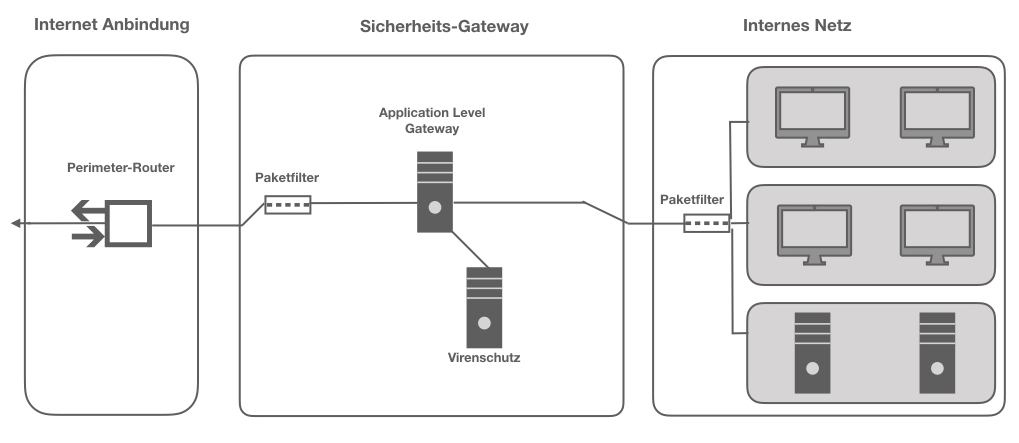
\includegraphics[width= \linewidth]{klUnternehmnorm}
	\caption{Grundarchitektur für ein kleines Unternehmen mit hohem Schutzbedarf}
	\label{klUhoch}
\end{figure}
	
	\chapter{Virtuelle LANs}

Virtuelle Netze oder auch virtuelle local area networks (VLAN) werden genutzt, um bestehende physische LANs in logische Abschnitte zu Unterteilen, oder auch um mehrere physische Netzabschnitte virtuell zu verbinden. VLANs werden mithilfe von Switches gebildet. Switche sind Netzwerkkomponenten, welche die Schichten eins und zwei des Internetprotokollstapels (vgl. Anhang \ref{A1}) implementieren, sie bilden heute die Zentralen Netzknoten in (lokalen) Netzwerken \cite{zisler2018computer}. 

%nutzen hinzufügen

\subsection{Funktionsweise}

% portbasiertes und tagged Vlan

Es gibt zwei Arten von Vlans, das Portbasierte und das Paketbasierte VLAN. 


	
	\chapter{Virtuelle Private Netzwerke}

Der Zugriff aus der Ferne auf das lokale Firmennetzwerk ist für verschiedene Anwendungsszenarien unabdingbar. Die Vernetzung von Firmenstandorten, der Zugriff von mobilen Mitarbeitern auf das Firmennetz oder auch ein Zugang für Geschäftspartner auf das Intranet des Unternehmens müssen sicher Umgesetzt werden.
Die Technologie, die dies ermöglichen soll ist \emph{VPN}. Ein VPN ist ein virtuelles privates Netz, eine logische Verbindung die auf einem anderen, physischen Netz aufgebaut wird \cite{zisler2018computer}. Grundsätzlich eignet sich jedes Netz, hier wird jedoch nur die Verwirklichung von VPN über das Internet betrachtet. Es wird unter anderem wird zwischen folgenden Varianten unterschieden:
\begin{itemize}
  \item Site-to-Site/ Branch Office VPN: Verbindung von verschiedenen Firmenstandorten,
  \item End-to-Site/ Remote Access VPN: Verbindung eines Heimarbeitsplatzes oder eines Mobilen Mitarbeiters it dem Intranet des Unternehmens.
  \item End-toEnd VPN: Verbindung zweier Endgeräte,
  \item Extranet VPN: gewährt einem Geschäftspartner/Kunden/Lieferanten Zugang zu Teilen des Internen Netzes 
\end{itemize}

Die Umsetzung des VPN kann entweder bei einem Dienstleister eingekauft werden, dies nennt sich \emph{Trusted VPN}, oder selber als \emph{secure VPN} aufgebaut werden. Beim Einsatz von Trusted VPN sollten vertrauliche Daten zusätzlich auf Anwendungsebene verschlüsselt werden, um sie zum Beispiel vor Innentätern des Dienstleisters zu schützen. 
 Es gibt außerdem Zwischenformen, so dass nur Teile der Technologie bei einem Dienstleister eingekauft werden.


\section{Funktionsweise}

Die Basistechnologie die einem VPN zugrunde liegt ist das \emph{Tunneling}. Es handelt sich um ein Verfahren, welches  Netzwerkprotokolle in beliebige andere Netzwerkprotokolle kapselt (\emph{encapsulation}), über ein Netzwerk verschickt und an einem gegebenen Endpunkt wieder auspackt (\emph{decapsulation}). Das Tunneling kann auf verschiedenen Schichten des Protokollstapels (vergl. Anhang \ref{A1}) ansetzten. Das Prinzip des Tunneling ist in Abbildung \ref{tunnel} dargestellt. Während der Übertragung durch das Internet ist für die Weiterleitung der Datenpakete nicht relevant, dass es sich um Pakete eines virtuellen Netzwerks handelt, hier werden nur die Header X und Y ausgewertet. Die Header A und B sind für den Transport außerhalb der Endpunkte des VPNs zu verwenden. Der Header de Tunneling-Protokolls gibt dem Empfänger am Endpunkt des Tunnels Informationen darüber, wie das Paket weiterzuleiten ist. 

\begin{figure}[h]
	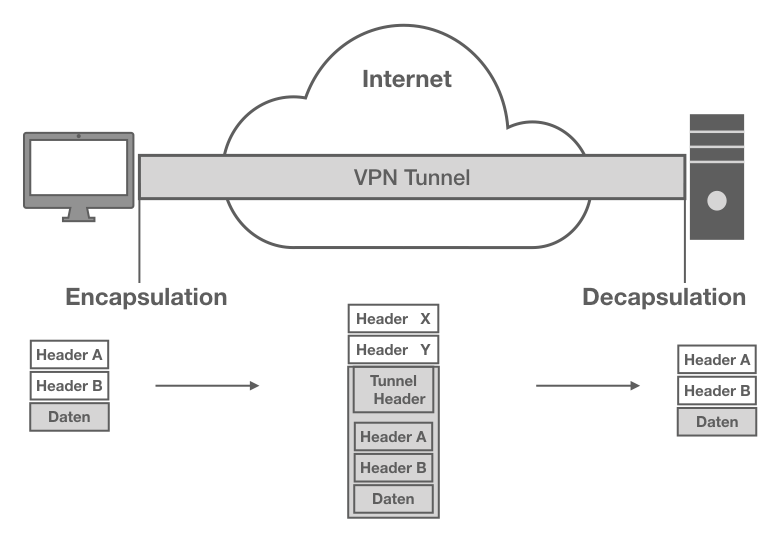
\includegraphics[width=\linewidth]{tunneling}
	\caption{Grundprinzip des Tunneling}
	\label{tunnel}
\end{figure}

 Im Folgenden sollen die wichtigsten standardisierten  Tunneling Protokolle zur VPN-Realisierung vorgestellt werden

\subsection{Layer-2-Protokolle}
Tunneling Protokolle die auf der Sicherungsschicht arbeiten....


\subsubsection{Layer 2 Tunneling Protocol (L2TP)}
Das L2TP ist der Nachfolger der Tunneling Protokolle PPTP (Point-to-Poit-Tunneling-Protokol) und L2F (Layer-two-Forwarding) \cite{isi-vpn}. Es kapselt Daten in PPP (Point-to-Point-Protocol \footnote{spezifiziert in RFC 1661: https://www.rfc-editor.org/rfc/rfc1661.txt}) Rahmen, ein Ende-zu-Ende Protokoll auf der Vermittlungsschicht, somit ist es möglich auch nicht-IP Pakete über das Internet zu transportieren \cite{gokulakrishnan2014survey}. Zur Authentisierung dienen die Protokolle EAP (Extensible Authentication Protocol) und CHAP (Challenge Handshake Protocol). Wobei CHAP nach \cite{eckert2018sicherheit}
Es können mehrere Verbindungen über einen einzigen L2TP Tunnel laufen, auch alle Management und Wartungsinformationen werden über diesen einen Tunnel ausgetauscht \cite{bohmer2005vpn}.
Da weder L2TP noch PPP die Vertraulichkeit der Daten gewähren, muss die Kommunikation zusätzlich abgesichert werden, dies wird häufig mit IPSec (siehe Abschnitt \ref{subsub:L3}) umgestzt. 
Das Haupteinsatzgeiet eines VPNs über L2TP ist ein Site-to-Site oder eines Telearbeitsplatzes.   

\subsection{Layer-3-Protokolle}
Bei Layer-3-Protokolle erfolgt die Kapselung der Daten auf der Vermittlungsschicht, auch Internetschicht oder Netzwerkschicht genannt. Ein Standardprotokoll zur Herstellung von VPN-Verbindungen auf dieser Ebene ist IPSec.
\subsubsection{Internet Protokol Security (IPSec)}
\label{subsub:L3}
Internet Protocol Security (IPSec) ist eine Protokollfamilie die drei Protokolle kombiniert, das IP Authentication Header (AH) zur Authentisierung, das Encapsulating Security Payload (ESP) ebenfalls zur Authentisierung und zur Verschlüsselung der Daten und das Internet Key Exchange (IKE) das zum Schlüsselaustausch und dem Verbindungsaufbau dient\footnote{Spezifiziert werden die Protokolle in den RFCs 4301,4302,4303 und 4306.}. Das AH und das ESP können einzeln oder zusammen genutzt werden. Da AH keine Verschlüsselung bietet ist für die Kommunikation über das Internet das ESP vorzuziehen. AH ist zur Authentifikation der Kommunikation in einem sicheren Netz geeignet \cite{isi-vpn}. Implementierungen von IPSec müssen deswegen ESP zur Verfügung stellen, die Einbindung von AH ist optional.

Sowohl für End-to-End, Site-to-Site und End-to-Site Verbindungen kann IPSec genutzt werden \cite{rfc4301}.

 Es gibt vielfältige Möglichkeiten IPSec zu konfigurieren, so ist zu beachten, dass es möglich ist ESP zu nutzen und dabei nur die Vertraulichkeit, nicht aber die Integrität sicherzustellen. Desweiteren besteht die Möglichkeit einen oder mehrere Tunnel für die Kommunikation zu nutzen. Die Sicherheit der Kommunikation  über IPSec ist abhängig von einer gewissenhaften Implementierung, Konfiguration und einer sicheren Systemumgebung \cite{rfc4301}. 
  
  IPSec ist sowohl für IPv4 als auch für IPv6 definiert, in IPv6 ist es bereits integriert.
\\

Es gibt zwei Benutzungsmodi: den Transportmodus und den Tunnelmodus. Im  Tunnelmodus kann ein klassisches VPN betrieben werden, hier werden IP-Pakete in anderen IP-Paketen gekapselt. Es wird also das gesamte IP-Paket geschützt, inklusive der getunnelten IP-Headerinformationen wie die tatsächliche Ziel und Absenderadresse. Ein Sicherheitsgateway, welches IPSec anbietet muss den Tunnelmodus implementieren und sollte auch dieses verwenden, der Transport von Daten im Transportmodus ist für Sicherheitsgateways nur in Ausnahmefällen erlaubt \cite{rfc4301}. 
\begin{figure}[h]
	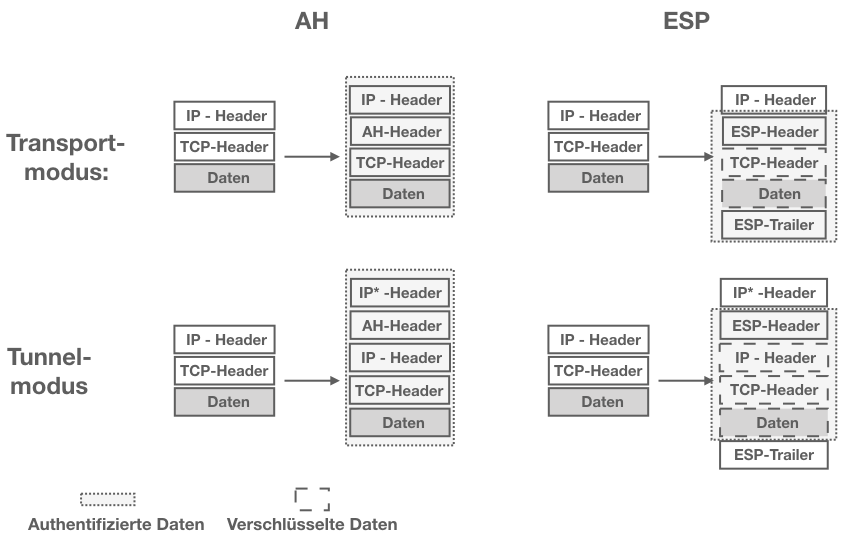
\includegraphics[width=\linewidth]{ahesp.001.png}
	\caption{Transportmodus und Tunnelmodus des IPSec nach \cite{lipp2007vpn}}
	\label{ahesp}
\end{figure}
Im Transportmodus werden die IP-Pakete nicht getunnelt sondern nur ihre Authentizitat und Integrität mittels AH gewährleistet oder zusätzlich die Vertraulichkeit mittels ESP. 

Abbildung \ref{ahesp} zeigt den Unterschied von Transport und Tunnelmodes anhand der Paketstruktur unter Benutzung von AH und ESP. 

 


\section{Sicherheitsmaßnahmen}



\section{Architektur}
Das VPN-Gateway kann an verschieden Stellen an das Netzwerk angeschlossen werden. Zu beachten ist

\begin{figure}[h]
	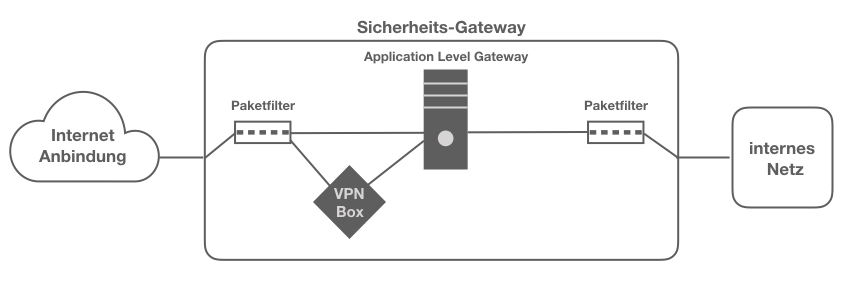
\includegraphics[width=\linewidth]{vpnarchitektur.jpeg}
	\caption{Sichere Einbindung eines VPN-Gateways in eine P-A-P Struktur}
	\label{vpnarch}
\end{figure}



\section{Anwendungsbereiche in privaten Haushalten}

Virtuelle private Netzwerke werden auch im privaten Bereich  verwendet. Hier gibt es hauptsächlich zwei Anwendungsszenarien: der Zugriff aus der Ferne auf das Heimnetzwerk zur Bedienung des IoT (Internet of Things) oder der Zugriff auf die NAS als Cloud-Alternative oder aber als Technologie zum Anonymen surfen im Internet oder zum Überwinden von Geoblocking. 







	
	\chapter{Zusammenfassung und Ausblick}

Ein Anstatz für die Verbesserung der IT-Sicherheit ist \emph{Security by Design}. Am Beispiel eines Netzwerkes sollten Vernetzung und Sicherheitsmaßnahmen nicht getrennt voneinander betrachtet werden, sondern ein Netzwerk aus intrisisch sicheren Komponenten Aufgebaut werden \cite{nicholson2018blurring}.
	
	\appendix
	
	\chapter{Anhang}
\section{Internetprotokollstapel}
\label{A1}
\begin{figure}[h]
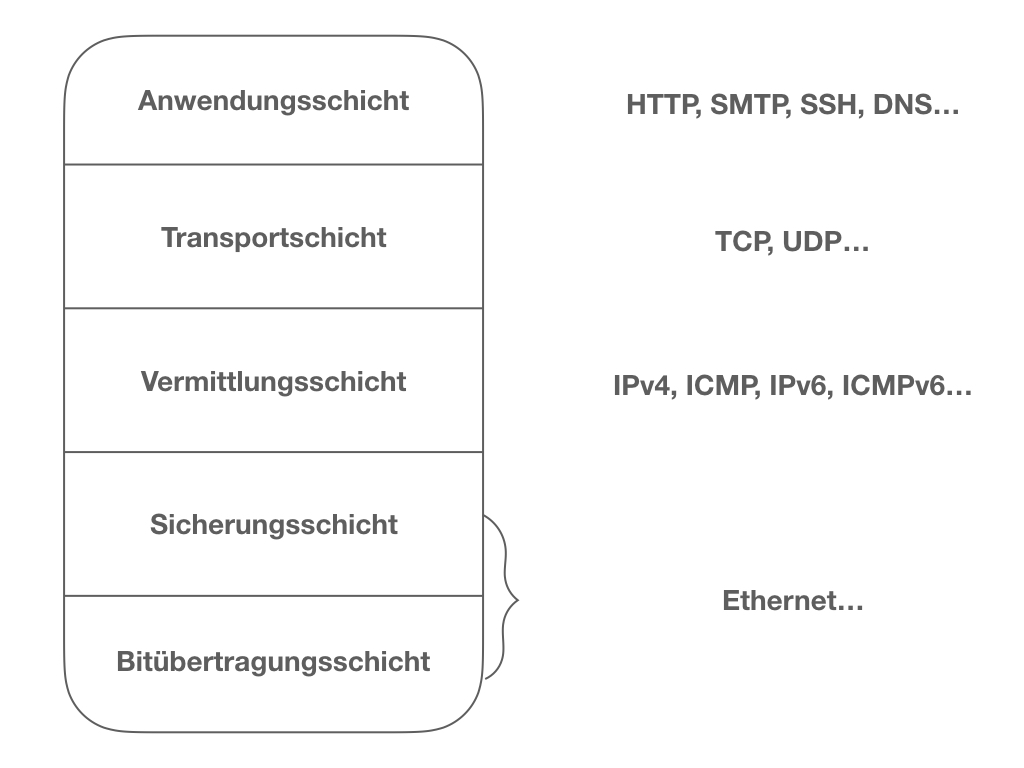
\includegraphics[width=\linewidth]{protstap}
\caption{Hybridmodell des Internetprotokollstapels}
\end{figure}
	

	%\nocite{*} % dient der Übersicht, sollte vor Abgabe entfernt werden
	\bibliography{it.bib}

\end{document}


